\documentclass[aspectratio=169]{beamer}
\usetheme{Madrid}
\usecolortheme{beaver}
\usepackage[utf8]{inputenc}
\usepackage[T1]{fontenc}
\usepackage{tikz}
\usepackage{amssymb}
\usepackage{graphicx}
\setbeamertemplate{navigation symbols}{}
\setbeamercolor{title}{fg=white,bg=cyan!60!black}
\setbeamercolor{frametitle}{fg=white,bg=cyan!50!black}
\setbeamercolor{block title}{bg=cyan!15,fg=black}
\setbeamercolor{block body}{bg=cyan!5,fg=black}

\title{G1 — Sprite Start}
\subtitle{Lesson 4: Three in a Row}
\author{ByteForge --- Grade 7 --- Game Maker}
\date{}

\begin{document}

\begin{frame}
    \titlepage
\end{frame}

\begin{frame}{Sequence — same Y, different X}
    \Large
    Three shapes "in a line" means one coordinate stays the SAME while the other changes — a huge amount of real layout is exactly this.

    \begin{center}
    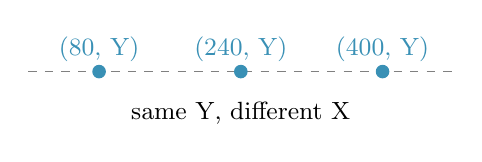
\begin{tikzpicture}[scale=0.9]

        \draw[dashed, gray] (0,-1) -- (6,-1);
        \filldraw[cyan!70!black] (1,-1) circle (2.5pt) node[above] {\small (80, Y)};
        \filldraw[cyan!70!black] (3,-1) circle (2.5pt) node[above] {\small (240, Y)};
        \filldraw[cyan!70!black] (5,-1) circle (2.5pt) node[above] {\small (400, Y)};
        \node[below] at (3,-1.3) {\small same Y, different X};
    \end{tikzpicture}
    \end{center}
\end{frame}

\begin{frame}{Your Turn}
    \Large
    Open the student map, find \textbf{G1 — Sprite Start}, and complete
    the \textbf{Three in a Row} challenge --- everything you just saw, they now do themselves.
\end{frame}

\end{document}
